\section{Neutral case}
\label{sec:ND_NeutralCase}
This section introduces a method to discretize properly
the surface layer of a simplified atmosphere column model.
First in \S \ref{sec:ND_NeutralCase_recallSplines},
the Finite Volume discretization using spline reconstruction
is recalled.
\S \ref{sec:ND_NeutralCase_strategies}
is an overview of several strategies used to deal
with the coupling of the two zones mentioned previously.
When it makes sense, the strategies are applied with a
Finite Volume discretization so that they can be
compared with each other.
Finally \S \ref{sec:ND_NeutralCase_newSFscheme}
introduces a new strategy to handle the surface flux scheme,
based on a logarithmic reconstruction of the profiles
within the surface layer.
\par
In this section \ref{sec:ND_NeutralCase},
we assume that the stratification is neutral.
As it was explained in Chapter \ref{ch:airseaSCM},
there is no effect of the stratification on the turbulent viscosity
so the wind speed $u(z, t)$ can be integrated in time
without the temperature and humidity profiles.
\subsection{Space discretization of
\eqref{eq:ND_NeutralCase_EkmanEq} with Finite Volumes}
\label{sec:ND_NeutralCase_recallSplines}
We recall here the Finite Volume discretization used throughout
this chapter. We focus on the space discretisation and the time
dependency of $u(z, t)$ is hence omitted.
\begin{figure}
	\centering
	\subimport{images/}{notations_FV.pdf_tex}
	\caption{Summary of the notations related to the discretisation.}
	\label{fig:ND_NeutralCase_summary_notations}
\end{figure}
\par
As already mentioned in chapter \ref{ch:approximatedDiscreteSchwarz}
the space domain is divided into $M$ cells delimited by
heights $(z_0=0, .., z_m, .., z_M)$. The size of the $m$-th cell
is $h_{m-\frac{1}{2}}=z_{m}-z_{m-1}$ and the average of $u(z)$
over this cell is noted
$\overline{u}_{m-\frac{1}{2}}=\frac{1} {h_{m-\frac{1}{2}}}
\int_{z_{m-1}}^{z_m}u(z)dz$.
The space derivative of $u$ at $z_m$ is noted $\phi_{m}$.
Figure \ref{fig:ND_NeutralCase_summary_notations} summarized
the notations used related to the discretisation.
Averaging \eqref{eq:ND_NeutralCase_EkmanEq} over a cell gives
the semi-discrete equation
\begin{equation}
\label{eq:ND_NeutralCase_semiDiscreteEkmanEq}
	(\partial_t + if) \overline{u}_{m+\frac{1}{2}} - 
	\frac{K_{u, m+1} \phi_{m+1} - K_{u, m} \phi_{m}}
		{h_{m+\frac{1}{2}}} = i f u_G
\end{equation}
The reconstruction of $u(z) = {\cal S}_{m+\frac{1}{2}}
				(z - z_{m+\frac{1}{2}})$
				inside a cell must be chosen
to pursue the derivation of the scheme. A simple choice is
a quadratic polynomial,
${\cal S}_{m+\frac{1}{2}}(\xi) = r_0 + r_1 \xi + r_2 \xi^2$ where
$-\frac{h_{m+1/2}}{2} \leq \xi \leq \frac{h_{m+1/2}}{2}$.
Averaging ${\cal S}_{m+\frac{1}{2}}$ over the cell and
prescribing its space derivative at $z_{m}$ and $z_{m+1}$
lead to the following system:
\begin{equation}
	\begin{aligned}
		\overline{u}_{m+1/2} &= \frac{1}{h_{m+1/2}}
		\int_{-\frac{h_{m+1/2}}{2}}^{\frac{h_{m+1/2}}{2}}
		{\cal S}_{m+\frac{1}{2}}(\xi)d\xi\\
		\phi_m &= \partial_z {\cal S}_{m+\frac{1}{2}}
		\left(-\frac{h_{m+1/2}}{2}\right)\\
		\phi_{m+1} &=
		\partial_z {\cal S}_{m+\frac{1}{2}}
		\left(\frac{h_{m+1/2}}{2}\right)
	\end{aligned}
\end{equation}
In matrix form, we obtain a system that can be inverted to
compute $r_0, r_1, r_2$:
\begin{equation}
    \begin{pmatrix}
    \overline{u}_{m+1/2} \\
    h_{m+\frac{1}{2}} \phi_m \\
	    h_{m+\frac{1}{2}} \phi_{m+1}
    \end{pmatrix} = 
    \begin{pmatrix}
    1 & 0 & \frac{1}{12} \\
    0 & 1 & -1 \\
    0 & 1 & 1 \\
    \end{pmatrix}
    \begin{pmatrix}
    r_0 \\
    r_1 h_{m+\frac{1}{2}} \\
    r_2 h_{m+\frac{1}{2}}^2
    \end{pmatrix}
\end{equation}
The reconstruction of $u(z)$ between $z_m$ and $z_{m+1}$
is then
\begin{equation}
\label{eq:ND_NeutralCase_quadraticReconstruction}
{\cal S}_{m+\frac{1}{2}}(\xi) =
	\Bar{u}_{m+\frac{1}{2}} + 
	\frac{\phi_{m+1}^{} + \phi_{m}^{}}{2} \xi
	+ \frac{\phi_{m+1}^{} - \phi_{m}^{}}{2h_{m+1/2}}
	\left(\xi^2 - \frac{h_{m+1/2}^2}{12}\right)
\end{equation}

The continuity of the solution at cell interfaces (${\cal S}_{m-\frac{1}{2}}\left(\frac{h_{m-1/2}}{2}\right) = {\cal S}_{m+\frac{1}{2}}\left(-\frac{h_{m+1/2}}{2}\right)$) is then equivalent to
%
\begin{equation}
\label{eq:ND_NeutralCase_continuityEquationFV}
	\frac{h_{m-1/2}}{\emphase{6}} \phi_{m-1} 
	+ \frac{\emphase{2}\frac{h_{m+1/2}+h_{m-1/2}}{2}}
		{\emphase{3}} \phi_m  
	+ \frac{h_{m+1/2}}{\emphase{6}} \phi_{m+1} = \Bar{u}_{m+\frac{1}{2}} - \Bar{u}_{m-\frac{1}{2}}
\end{equation}
Combining \eqref{eq:ND_NeutralCase_semiDiscreteEkmanEq}
and \eqref{eq:ND_NeutralCase_continuityEquationFV} finally gives
the prognostic equation to integrate
$\partial_z u$ in time:
\begin{equation}
\begin{aligned}
\label{eq:ND_NeutralCase_prognosticEqFV}
	(\partial_t + if) &\left( \frac{h_{m-\frac{1}{2}}}{6}
				\phi_{m-1}
	+ \frac{h_{m-\frac{1}{2}} + h_{m+\frac{1}{2}}}{3} \phi_m
	+ \frac{h_{m+\frac{1}{2}}}{6} \phi_{m+1} \right) \\
	&-
    \left(
	%\frac{K_{u, m+1}}{ h_{m+\frac{1}{2}}}\phi_{m+1} -
	%\frac{(h_{m-\frac{1}{2}} + h_{m+\frac{1}{2}}) K_{u,m}}{h_{m-\frac{1}{2}} h _{m+\frac{1}{2}}}\phi_m +
	%\frac{K_{u,m-1}}{h_{m-\frac{1}{2}}}\phi_{m-1}
	\frac{K_{u, m+1}\phi_{m+1} - K_{u, m}\phi_{m}}{ h_{m+\frac{1}{2}}} -
	\frac{K_{u, m}\phi_{m} - K_{u,m-1}\phi_{m-1}}{h_{m-\frac{1}{2}}}
    \right)
= 0
\end{aligned}
\end{equation}
To reconstruct the solution, $\overline{u}$ should also be 
integrated in time with \eqref{eq:ND_NeutralCase_semiDiscreteEkmanEq}.
\eqref{eq:ND_NeutralCase_prognosticEqFV} and
\eqref{eq:ND_NeutralCase_semiDiscreteEkmanEq} are hence the two 
equations defining our finite volume discretization.
Note that we arrive naturally on fourth-order compact schemes for
the first derivative $\partial_z u$
(eq \eqref{eq:ND_NeutralCase_continuityEquationFV})
and second-order for
$\partial_z^2 u$ (see e.g. \cite{piller_finite-volume_2004}),
but with a different approach of imposing a spline reconstruction.
This approach lets us better control the vertical profiles
than the usual compact methods and
facilitates the derivation of the boundary conditions.
\paragraph{Remark: fourth-order compact scheme}
To get a more accurate scheme for the second-order derivative,
a fourth degree polynomial could also be used.
if $\frac{1}{12}, \frac{5}{6}$ are used in
\eqref{eq:ND_NeutralCase_prognosticEqFV} instead of
$\frac{1}{6}, \frac{2}{3}$, a fourth-order compact scheme
is obtained. This scheme is studied in the Finite Difference sense
in \citep{adam_highly_1977} and was also used
by \cite{piller_finite-volume_2004} in a Finite Volume framework
close to the one we are using.
If one assumes that the reconstruction is the fourth degree
polynomial
${\cal S}_{m+\frac{1}{2}}^4(\xi) = r_0^4 + r_1^4 \xi + r_2^4 \xi^2 
+ \emphase{r_3^4 \xi^3} + \emphase{r_4^4 \xi^4}$,
the two additional degrees of freedom $\emphase{r_3^4},
\emphase{r_4^4}$ need to be
constrained. To recover the fourth-order compact scheme through
the continuity constraint as in
\eqref{eq:ND_NeutralCase_continuityEquationFV}
one must put as constraints that the
reconstruction on the boundaries of the cell is
${\cal S}^4_{m+\frac{1}{2}}\left(\frac{h_{m+\frac{1}{2}}}{2}\right) =
\overline{u}_{m+\frac{1}{2}} +
\frac{h_{m+\frac{1}{2}}}{\emphase{12}}\left(
\phi_m + \emphase{5}\phi_{m+1}\right) $ and
${\cal S}^4_{m+\frac{1}{2}}\left(-\frac{h_{m+\frac{1}{2}}}{2}\right) =
\overline{u}_{m+\frac{1}{2}} -
\frac{h_{m+\frac{1}{2}}}{\emphase{12}}\left(
\emphase{5}\phi_m + \phi_{m+1}\right)$.
Then the reconstruction is given by
\begin{equation}
    \begin{pmatrix}
    r_0^4 \\
    r_1^4 h_{m+\frac{1}{2}} \\
    r_2^4 h_{m+\frac{1}{2}}^2 \\
    r_3^4 h_{m+\frac{1}{2}}^3 \\
    r_4^4 h_{m+\frac{1}{2}}^4
    \end{pmatrix}
     = 
    \begin{pmatrix}
    1 & 0 & \frac{1}{12} & 0 & \frac{1}{80} \\
    0 & 1 & -1 & \frac{3}{4} & -\frac{1}{2} \\
    0 & 1 & 1 & \frac{3}{4} & \frac{1}{2} \\
    1 & -\frac{1}{2} & \frac{1}{4} & -\frac{1}{8}
    & \frac{1}{16} \\
    1 & \frac{1}{2} & \frac{1}{4} & \frac{1}{8}
    & \frac{1}{16} \\
    \end{pmatrix}^{-1}
    \begin{pmatrix}
    \overline{u}_{m+1/2} \\
    h_{m+\frac{1}{2}} \phi_m \\
	    h_{m+\frac{1}{2}} \phi_{m+1} \\
	    \overline{u} - \frac{5}{12} h_{m+\frac{1}{2}} \phi_m
	    - \frac{1}{12} h_{m+\frac{1}{2}} \phi_{m+1} \\
	    \overline{u} + \frac{1}{12} h_{m+\frac{1}{2}} \phi_m
	    + \frac{5}{12} h_{m+\frac{1}{2}} \phi_{m+1}
    \end{pmatrix}
\end{equation}
and one obtains a subgrid reconstruction corresponding to
the fourth-order
\footnote{
On the domain boundaries there is no continuity constraint.
${\cal S}^4_{\frac{1}{2}}\left(-\frac{h_{\frac{1}{2}}}{2}\right)$
can be constrained by a special treatment
(see \cite{piller_finite-volume_2004})
to keep the fourth-order accuracy on Dirichlet boundaries.
}
compact scheme considered.
However this representation is heavier than using the quadratic
splines: the fourth-order compact scheme will not be used in the
following.
\subsection{State-of-the-art surface flux schemes}
\label{sec:ND_NeutralCase_strategies}
We present in this subsection several strategies to derive the
discretization of the surface layer (the corresponding equation
is \eqref{eq:ND_NeutralCase_ConstantFlux}).
A surface layer discretization consists in two parts,
corresponding to the two steps of the integration in time
presented in Section \ref{sec:ND_Intro_continuousModel}:
\begin{itemize}
	\item how $u_\star$ is computed.
		For instance, with Finite Differences
		$u(\delta_{\rm sl}, t^n)$ is 
		used as an input of the
		bulk routine to get the value of
		$u_\star = BULK(u(\delta_{\rm sl}, t^n))$.
	\item How \eqref{eq:ND_NeutralCase_ConstantFlux}
		is implemented as
		a boundary condition: in particular,
		the height at which the flux is prescribed.
		The space discretisation of
		$u(\delta_{\rm sl}, \cdot)$ is the same
		in the bulk routine and in
		$e_\tau= \frac{u(\delta_{\rm sl},
		t^{n+1})}
		{||u(\delta_{\rm sl}, t^n)||}$.
\end{itemize}
\cite{nishizawa_surface_2018} investigated the effect of the
first part of the discretization and showed that there is a
negative bias in conventional surface flux schemes. This
bias comes from the fact that these schemes assume that the
volume-averaged variables are equal to the value in the center
of the volume. However the prognostic variables in the surface layer
follow a logarithmic profile as shown in
\eqref{eq:ND_NeutralCase_WallLaw}: the concavity of this profile thus
creates a systematic error when assuming that the average and the
value at the center of the cell are equal
(see Figure \ref{fig:ND_NeutralCase_nishizawaBias}).
\begin{figure}
	\centering
	\subimport{images/}{Nishizawa_bias.pdf_tex}
	\caption{The averaged value of the wall law is
		systematically smaller that the value at
		the center of the cell.}
	\label{fig:ND_NeutralCase_nishizawaBias}
\end{figure}
Finally, \cite{nishizawa_surface_2018} propose an alternative
bulk formulation which uses the averaged variable in the surface layer
instead of its value at the top.
\begin{remark}
The scheme \eqref{eq:ND_NeutralCase_prognosticEqFV} based
	on quadratic spline reconstruction is particular. \myTD{ca veut dire quoi ???}
The value at the center of the first cell is
		\begin{equation}
			{\cal S}_{1/2}(0) = \overline{u}_{1/2}
			+ \frac{h_{1/2}}{24} (\emphase{\phi_0-\phi_1})
		\end{equation}
 If $\phi_0$ and $\phi_1$ are aligned with $e_\tau=1+0i$ then
	$\phi_0 > \phi_1$ implies that $u(z)$ is concave
	(it is parabolic) and
	that $\overline{u}_{1/2} < {\cal S}_{1/2}(0)$.
	However, as it will be discussed in \S
	\ref{sec:ND_NeutralCase_newSFscheme}
	("On the value of $K_{u,0}$")
	the wall law cannot be followed.
	The modification of $K_{u,0}$ used in \S
	\ref{sec:ND_NeutralCase_newSFscheme} reduces
	the difference between $\overline{u}_{1/2}$
	and ${\cal S}_{1/2}(0)$.
	In the following, the
	difference between "FV pure" and "FV1"
	will be small for this reason.
\end{remark}
%
Our objective is to compare this\myTD{lequel?} surface flux scheme with the
conventional ones
and to introduce another surface flux scheme that is more coherent
with respect to the continuous model of Section
\ref{sec:ND_Intro_continuousModel}.
We now present the strategies that are representative of
what is done in actual models. The strategies are applied to
the Finite Volume scheme presented in Section
\ref{sec:ND_NeutralCase_recallSplines} and are
summarized in Figure \ref{fig:ND_NeutralCase_summary_sfscheme}.
  \begin{itemize}
	  \item With Finite Differences:
		  it is assumed that
		  $\delta_{\rm sl} = z_{\frac{1}{2}}$.
		A standard Finite Difference approximation applied to
		  the evolution equation states that
		  $(\partial_t+if) u_{\frac{1}{2}}
		  =\frac{1}{h_{\frac{1}{2}}}(K_1\phi_1 - K_0\phi_0)
		  + if u_G$.
		  The input value of the bulk is
		  $u(\delta_{sl}) = u_{1/2}$ and the boundary
		  condition is simply applied on the surface flux:
		\begin{equation}
			\underbrace{K_{u,0}
			\emphase{\phi}^{n+1}_\emphase{0}}_{\text{Surface flux}}
		= u_\star^2 e_\tau, ~~~~~~~~
			u_\star = {\rm BULK}(
			\underbrace{u_{\frac{1}{2}}^{n}}_{
				\text{FD value at }
			z_{\frac{1}{2}}})
		\end{equation}
		  Note that using another point further from
		  the surface (e.g. $u_{\frac{7}{2}}^n$) instead
		  of $u_{\frac{1}{2}}^n$ is the idea of the method
		  given by \citep{kawai_wall-modeling_2012}
		  to eliminate log-layer mismatch in LES models.
		  We do not consider this method here as we focus
		  on Finite Volume discretisation.
	  \item "FV pure": it is assumed again that
		  $\delta_{\rm sl} = z_{\frac{1}{2}}$.
		  The scheme is similar to the Finite Difference one.
	    The reconstruction of $u(z)$ inside the first grid cell
		  is used to get $u(z_{\frac{1}{2}})$.
		  The first cell is treated like the others:
		  \eqref{eq:ND_NeutralCase_EkmanEq} is
		  applied inside the surface layer.
	The bottom boundary condition is
	\begin{equation}
		\underbrace{K_{u,0} \emphase{\phi}^{n+1}_\emphase{0}}_{\text{Surface flux}}
		= u_\star^2 e_\tau, ~~~~~~~~
			u_\star = {\rm BULK}(
			\underbrace{{\cal S}_{1/2}^{n}(\xi=0)}_{
				\text{Reconstruction at }
			z_{\frac{1}{2}}})
	\end{equation}
		  Note that $\xi=0$ corresponds here
		  to $z=z_{\frac{1}{2}}\neq 0$.
	  \item "FV1": it is assumed again that
		  $\delta_{\rm sl} = z_{\frac{1}{2}}$.
		  In state-of-the-art models using finite volumes,
		  $u_{\star}$ is often computed using the
		  volume-averaged value
		  $u(\delta_{sl}) = \overline{u}_{\frac{1}{2}}$.
		  \eqref{eq:ND_NeutralCase_EkmanEq} is
		  also applied inside the surface layer.
		The corresponding bottom boundary condition is
		  \begin{equation}
		\underbrace{K_{u,0} \emphase{\phi}^{n+1}_\emphase{0}}_{\text{Surface flux}}
		= u_\star^2 e_\tau, ~~~~~~~~
			u_\star = {\rm BULK}(
			\underbrace{\overline{u}^{n}_{\frac{1}{2}}}_{
				\text{Average around }
			z_{\frac{1}{2}}})
		  \end{equation}
\end{itemize}
We present now two additional strategies corresponding to
the treatment of the surface layer in \citep{nishizawa_surface_2018}.
\begin{itemize}
    \item "FV Nishizawa":  unlike the other strategies,
	    it is assumed that the first cell is entirely inside
		the surface layer: $\delta_{\rm sl} = z_{1}$.
		We mentioned previously that
		\cite{nishizawa_surface_2018} show that the "FV1"
		strategy systematically underestimates
		$u(\delta_{\rm sl})$ because of the
	  concavity of the logarithmic profile.
	  An alternative bulk algorithm is hence derived by averaging
		\eqref{eq:ND_NeutralCase_WallLaw} in the first cell:
	\begin{equation}
		||\overline{u}_{\frac{1}{2}}||
		= \frac{u_\star}{\kappa}
		\left(1\emphase{+\frac{z_u}{\delta_{sl}}}\right)
		\left(\ln(1+\frac{z}{z_u})\emphase{-1}\right)
	\end{equation}
	However, the equation \eqref{eq:ND_NeutralCase_EkmanEq}
	and the spline reconstruction are left unchanged in the
	surface layer:
		  \begin{equation}
		\underbrace{K_{u,0} \emphase{\phi}^{n+1}_\emphase{0}}_{\text{Surface flux}}
		= u_\star^2 e_\tau, ~~~~~~~~
			  u_\star = \underbrace{\overline{{\rm BULK}}(}_{
				  \text{Adapted for averages}}
			  \overline{u}^{n}_{\frac{1}{2}}~~)
		  \end{equation}
	\item "FV2": the "FV Nishizawa" scheme is not adapted to
		spline reconstruction. We extend it to our
		Finite Volume discretisation with the assumption
		that the spline reconstruction $u(z)$ inside
		the surface layer is given by the wall law.
	    The surface layer \textit{is} the first cell:
	    the equation \eqref{eq:ND_NeutralCase_EkmanEq}
	    is not integrated in time in this cell
	and we use instead the wall law
	\eqref{eq:ND_NeutralCase_WallLaw} between 0 and
		$\delta_{sl} = z_1$.
	Since the profile of $u$ is given by the wall law
	in the first cell,
	using $\overline{u}_{\frac{1}{2}}$ as input of
	the alternative bulk algorithm of "FV Nishizawa"
	becomes rigorously equivalent to using the
	classical bulk formulation with $u(z_1)$
	as input.
	We hence use the reconstruction
	$u^n(\delta_{\rm sl}) = {\cal S}^n_{\frac{3}{2}}(
	  -\frac{h_{3/2}}{2})$ and the boundary condition
		  at $z_1$ is
	  \begin{equation}
		\underbrace{K_{u,1} \emphase{\phi}^{n+1}_\emphase{1}}_{\text{Flux at } z_1}
		= u_\star^2 e_\tau, ~~~~~~~~
			  u_\star = \underbrace{\overline{{\rm BULK}}(
			  \overline{u}^{n}_{\frac{1}{2}})}_{
				  \text{Averaged bulk}
			  } = {\rm BULK}(
			\underbrace{{\cal S}_{3/2}^{n}
			(\xi=-\frac{h_{\frac{3}{2}}}{2})}_{
				\text{Reconstruction at }
			z_{1}})
		  \end{equation}
	The first cell is inactive with this method:
	the numerical computation domain matches with the continuous
	one (Figure \ref{fig:ND_NeutralCase_EkmanContinuous}).
  \end{itemize}
  % Note that for the first two strategies "FV pure" and
  % "FV1", for numerical reasons $K_{u,0}$
  % should not actually
  % take the value $\left. K_{u}\right|_{z=0} = K_{mol}$.
  % See section \ref{sec:ND_StratifiedCase_viscosity0_FVpure} for
  % the explanation.
\begin{figure}
	\centering
	\subimport{images/}{sf_scheme_strategies.pdf_tex}
	\caption{Summary of the surface flux schemes.
	Averaged values are noted with vertical dotted lines;
	Values considered in the Finite Difference
	sense are encircled; implicit parts of the schemes
	are represented as dashed lines; orange profiles
	follow the wall law.
	With "FV Nishizawa", the average is \textit{interpreted}
	as the average of a wall law and is used in the
	$\overline{\rm BULK}$ routine.
	}
	\label{fig:ND_NeutralCase_summary_sfscheme}
\end{figure}
The different strategies are summarized in Table
\ref{tab:ND_NeutralCase_summary_sfscheme} together with the
"FV free" scheme which will be presented in \S
\ref{sec:ND_NeutralCase_newSFscheme}.
Let us draw some comments and comparisons on the surface flux schemes:
\begin{itemize}
	\item "FV1" relies on the assumption that
		$\overline{u}_{\frac{1}{2}} = u(z_{\frac{1}{2}})$;
		as it will be seen on Figure
		\ref{fig:ND_NeutralCase_comparisonPlot} the
		induced difference with "FV pure" is not important
		in our case where the spline profile are less concave
		than the logarithmic profile.
		We will thus only consider "FV pure" to
		reduce the number of cases.
	\item Some of the strategies assume
		\eqref{eq:ND_NeutralCase_EkmanEq} inside the surface
		layer; it is not satisfactory because it is
		incompatible with the wall law
		\eqref{eq:ND_NeutralCase_ConstantFlux}.
		Note that this is not
		the case with Finite Differences:
		$\eqref{eq:ND_NeutralCase_EkmanEq}$ is only assumed
		at $z_{1/2}$.
	\item With our spline reconstruction, when we assume
		\eqref{eq:ND_NeutralCase_EkmanEq} a spline
		profile (that is incompatible
		with the logarithmic profile) is also assumed.
\end{itemize}
As shown in Table \ref{tab:ND_NeutralCase_summary_sfscheme}
the "FV2" surface flux scheme solves those problems.
However for this scheme and all the others presented here,
changing the space step
also changes the height of the surface layer $\delta_{\rm sl}$.
This behaviour is not satisfactory: although
the choice of $\delta_{\rm sl}$ is mainly related to numerical
reasons we aim to approximate the continuous equations
\eqref{eq:ND_NeutralCase_continuousModel}.
\cite{basu_cautionary_2017} warns that using a small space step
while keeping the same treatment in LES goes against the
range of validity of the MOST profiles.
That is why in the following,
we derive a surface flux scheme that keeps
the advantages of the "FV2" scheme, but with a free $\delta_{\rm sl}$.
%
\begin{table}
	\centering
\begin{tabular}{c|c|c|c|c}
	Scheme & SL flux & $u_\star$ & $\delta_{sl}$ 
		& \eqref{eq:ND_NeutralCase_ConstantFlux} in SL? \\
		\hline
		FD & $K_{u,0} \phi_0$ & ${\rm BULK}(u_{\frac{1}{2}})$
			& $z_{\frac{1}{2}}$ & \checkmark \\
		"FV pure" & $K_{u,0} \phi_0$ &
			${\rm BULK}({\cal S}_{1/2}^{n}(\xi=0))$
			& $z_{\frac{1}{2}}$ & $\times$ \\
		"FV1" & $K_{u,0} \phi_0$ &
			${\rm BULK}(\overline{u}_{\frac{1}{2}})$
			& $z_{\frac{1}{2}}$ & $\times$ \\
		"FV Nishizawa" & $K_{u,0} \phi_0$ &
			$\overline{\rm BULK}
				(\overline{u}_{\frac{1}{2}})$
			& $z_1$ & $\times$ \\
		"FV2" & $K_{u,1} \phi_1$ &
			${\rm BULK} ({\cal S}_{\frac{3}{2}}(
				  -\frac{h_{3/2}}{2}))$
			& $z_1$ & \checkmark \\
		"FV free" & $K_{u,\delta} \phi_{\delta}$ &
			${\rm BULK}
				(u(\delta_{sl}))$
			& $\delta_{sl}$ & \checkmark \\
	\end{tabular}
	\caption{Summary of the surface flux schemes presented in
	Section \ref{sec:ND_NeutralCase}}
	\label{tab:ND_NeutralCase_summary_sfscheme}
\end{table}
\subsection{A surface flux scheme with a free $\delta_{\rm sl}$}
\label{sec:ND_NeutralCase_newSFscheme}
We now construct a boundary condition that is coherent
with the continuous model presented in
\S \ref{sec:ND_Intro_continuousModel}
with a free $\delta_{sl}$, named "FV free" in Table
\ref{tab:ND_NeutralCase_summary_sfscheme}:
\begin{equation}
	\label{eq:ND_NeutralCase_bottomCondFVFree}
	\underbrace{K_{u,\delta}
	\emphase{\phi}^{n+1}_\emphase{\delta}}_{\text{Flux at }
	\delta_{sl}}
		= u_\star^2 e_\tau, ~~~~~~~~
			  u_\star = {\rm BULK}(
			\underbrace{u^n(\delta_{\rm sl})}_{
				\text{Reconstruction at }
			\delta_{sl}})
\end{equation}
We first assume
that $\delta_{\rm sl} < z_1$ and will then relax this hypothesis.
In the first grid cell, we assume that
\eqref{eq:ND_NeutralCase_WallLaw} applies for $z<\delta_{sl}$
and we separate the 
first volume into two parts: the surface layer $[0,\delta_{\rm sl}]$ and the "sub-cell" $[\delta_{\rm sl}, z_1]$.
This split corresponds to the change of governing equations
in the continuous case \eqref{eq:ND_NeutralCase_continuousModel}.
Let $\widetilde{h} = z_1 - \delta_{\rm sl}$  be the size of the
upper sub-cell $[\delta_{\rm sl}, z_1]$
and $\widetilde{u} = \frac{1}{\widetilde{h}}\int_{\delta_{sl}}^{z_1}
u(z)dz$ be the averaged value of $u$ on this interval.
The following subgrid reconstruction is used:
\begin{equation}
	\label{eq:ND_NeutralCase_fullReconstruction}
	u(z) = \begin{cases} \displaystyle
		\emphase{{\cal S}_{1/2}}\left(z - \frac{z_1 +
				\delta_{sl}}{2}\right),
		~~~~~~~~~~~ z \geq \delta_{sl}
		\\ \displaystyle
		\frac{{u_\star}}{\kappa}
		\ln(1+\frac{z}{z_{u}})e_\tau,% + u(0),
		~~~ z < \delta_{sl}
	\end{cases}
\end{equation}
The quadratic spline $\emphase{{\cal S}_{1/2}}$ used for reconstruction
is computed with the averaged value $\widetilde{u}$, the
size of the sub-cell $\widetilde{h}$ and the fluxes at the
extremities $\phi_{\delta}$ and $\phi_1$:
a similar equation to
\eqref{eq:ND_NeutralCase_quadraticReconstruction}
is obtained:
$\emphase{{\cal S}_{1/2}}(\xi) = 
\emphase{\widetilde{\color{black} u}} +
\frac{\phi_{1} + \phi_\emphase{\delta}}{2} \xi
+ \frac{\phi_{1} -
\phi_\emphase{\delta}}{2\emphase{\widetilde{\color{black} h}}}
\left(\xi^2 - \frac{\emphase{\widetilde{\color{black} h}}^2}{12}\right)$.
The notations are summed up in Figure
\ref{fig:ND_NeutralCase_nouvelle_dis_neutre}.
\begin{figure}
	\subimport{images/}{nouvelle_dis_neutre.pdf_tex}
	\caption{ Surface layer scheme "FV free".}
	\label{fig:ND_NeutralCase_nouvelle_dis_neutre}
\end{figure}
\begin{remark}
	The flux $K_u \phi$ is constant in the surface layer. Hence
	$K_{u,\delta}\phi_{\delta} = K_{u,0} \phi_0$ and since the
	viscosity at $z=0$ is the molecular viscosity we get
	$\phi_{\delta} = \frac{K_{mol}}{K_{u,\delta}} \phi_0$.
	The implementation uses $\phi_{\delta}$ as a prognostic
	variable instead of $\phi_0$:
	this surface flux scheme is hence exactly equivalent
	to using the "FV2" scheme with grid levels
	$\{0, \delta_{sl}, z_1, z_2, ..., z_M\}$.
\end{remark}
\par
We now rewrite the reconstruction
\eqref{eq:ND_NeutralCase_fullReconstruction} in terms
of the prognostic variables $\overline{u}_{1/2}$, $\phi_\delta$,
$\phi_1$.
The relation between $\overline{u}_{1/2}$ and $\widetilde{u}$ is 
given by the Chasles' relation
$ \int_{\delta_{sl}}^{z_1} u dz = \int_{z_0}^{z_1} u dz -
\int_{z_0}^{\delta_{sl}} u dz$, which can be written as
\begin{equation}
\label{eq:ND_NeutralCase_Chasles}
	\widetilde{h}\emphase{\widetilde{u}} =
	h_{1/2}\emphase{\overline{u}_{1/2}} -
	\emphase{e_\tau} \frac{{u_\star}}{\kappa}\int_{z_0}^{\delta_{sl}}
	\ln(1+\frac{z}{z_{u}}) dz
	%+ (\delta_{sl}-z_0) u(0)
\end{equation}
where the time indices in
$e_\tau = \frac{u^\emphase{n+1}(\delta_{sl})}
{||u^\emphase{n}(\delta_{sl})||}$ must be the same as in the
bottom boundary condition
\eqref{eq:ND_NeutralCase_bottomCondFVFree}.
Let us inject the reconstruction of
$u(\delta_{sl}) = \widetilde{u} - \widetilde{h}(\phi_{\delta}/3 + \phi_1/6)$
(obtained from \eqref{eq:ND_NeutralCase_fullReconstruction})
and the log law $||u^n(\delta_{sl})|| = \frac{{u_\star}}{\kappa}\ln(1+\frac{\delta_{sl}}{z_{u}})$ in \eqref{eq:ND_NeutralCase_Chasles}.
One then gets:
\begin{equation}
	\label{eq:ND_NeutralCase_utildeExpression}
	% \frac{\widetilde{h}}{h_{1/2}}\widetilde{u} = \overline{u}_{1/2} - \left(\widetilde{u} - \widetilde{h}(\phi_{\delta}/3 + \phi_1/6)
	% \right)\tau_{sl} +
	% (\tau_{sl} - \frac{h_{1/2} - \widetilde{h}}{h_{1/2}})u(0)
	\emphase{\widetilde{u}} \; \alpha_{sl} =
	\emphase{\overline{u}_{\frac{1}{2}}} + \widetilde{h}\left(
	\frac{\emphase{\phi_\delta}}{3} + \frac{\emphase{\phi_1}}{6} \right)
	\left(\alpha_{sl} - \frac{\widetilde{h}}{h_{\frac{1}{2}}}\right)
\end{equation}
\myTD{J'aèrerais un peu}
with $\alpha_{sl} =
\frac{\widetilde{h}}{{h_{1/2}}} + \frac{1}{{h_{1/2}}}\int_{z_0}^{\delta_{sl}}
\frac{\ln(1+\frac{z}{z_{u}})}{\ln(1+\frac{\delta_{sl}}{z_{u}})}dz
= \frac{(h_{1/2} + z_{u})
\ln(1+\frac{\delta_{\rm sl}}{z_{u}}) - \delta_{\rm sl}}{
	h_{1/2}\ln(1+\frac{\delta_{sl}}{z_{u}})}$ a non-dimensional
number $0 < \alpha_{sl} \leq 1$ which depends on the log law and
on the values of $\widetilde{h}, h_{1/2}$. It decreases with
$\delta_{sl}$; $\alpha_{\rm sl} = 1 \iff \widetilde{h}=h_{1/2}$
and in this case \eqref{eq:ND_NeutralCase_utildeExpression} is
equivalent to $\widetilde{u} = \overline{u}_{1/2}$.
Figure \ref{fig:ND_NeutralCase_alpha_sl} shows the
profile of $\alpha_{sl}$.
\begin{figure}
	\centering
	\includegraphics[scale=0.7]{images/alpha_sl.pdf}
	\caption
	{ Value of $\alpha_{sl}$
	for several values of $z_u$ with $z_1=20\;{\rm m}$.
	}
	\label{fig:ND_NeutralCase_alpha_sl}
\end{figure}
\begin{remark}
$\alpha_{\rm sl}$ is a constant in the neutral case
only when $\delta_{\rm sl}$ and $z_{u}$ are constants. However
$z_{u}$ depends on $u_\star$ and will vary.
In all this thesis we assume that $\delta_{\rm sl}$ does not
change over time.
	\myTD{d'autre part, + commentaires (+ paramètre physique ?)}
\end{remark}
%
In the reconstruction \eqref{eq:ND_NeutralCase_fullReconstruction}
$\widetilde{u}$ can be expressed in terms of the prognostic
variables with \eqref{eq:ND_NeutralCase_utildeExpression}
and we obtain $u(\delta_{sl})$ which is used as input
of the bulk routine and in the computation of $e_\tau$:
\begin{equation}
u(\delta_{sl})=\frac{\overline{u}_{1/2} -
	\frac{\widetilde{h}^2}{h_{1/2}}
	(\frac{\phi_{\delta}}{3} + \frac{\phi_1}{6})}
	{\alpha_{\rm sl}}
\end{equation}
The boundary condition \eqref{eq:ND_NeutralCase_bottomCondFVFree}
is hence formulated as:
\begin{equation}
	\label{eq:ND_NeutralCase_boundaryCondFVfree}
	\underbrace{K_{u,\delta} {\phi}^{n+1}_{\delta}}_{
		\text{Flux at } \delta_{sl}
	} = u_\star^2
	\underbrace{\frac{\overline{u}_{1/2} -
	\frac{\widetilde{h}^2}{h_{1/2}}
	(\frac{\phi_{\delta}}{3} + \frac{\phi_1}{6})}
	{\alpha_{\rm sl}||u^n(\delta_{sl}) ||}}_{
		e_\tau \text{ using reconstruction at } \delta_{sl}
	}
\end{equation}
and the evolution equation in the upper part of the first grid level
$ (\partial_t+if) \emphase{\widetilde{u}}
= \frac{K_{u, 1}\phi_1 - K_{u,\delta} \phi_{\delta}}{\widetilde{h}}$
becomes
\begin{equation}
	\label{eq:ND_NeutralCase_semiDiscreteEkmanEqFVfree}
	(\partial_t+if) \left(\frac{1}{\alpha_{\rm sl}(t)}
	\left(\overline{u}_{1/2} + \widetilde{h}
	\left(\frac{\phi_{\delta}}{3} + \frac{\phi_1}{6}\right)
	\left(\alpha_{sl} - \frac{\widetilde{h}}{h_{\frac{1}{2}}}\right)
	%+ (\alpha_{sl} - 1) u(0)
	\right)\right)
	= \frac{K_{u, 1}\phi_1 - K_{u,\delta} \phi_{\delta}}{\widetilde{h}}
\end{equation}
The prognostic equation \eqref{eq:ND_NeutralCase_continuityEquationFV}
used to integrate $\phi$ in time
is also changed for $m=1$: $h_{m-1/2}$ is replaced
with $\widetilde{h}$ and $K_{u, m-1}\phi_{m-1}$ is replaced by
$K_{u,\delta}\phi_{\delta}$.
%
\begin{figure}[htpb]
	\centering
	\includegraphics[scale=0.6]{images/neutral_comparisonPlot.pdf}
	\caption[Vertical profiles of $|u|$ and $\arg(u)$]
	{Vertical profiles of $||u||$ (left) and $\arg(u)$ (right)
	for the various surface flux schemes presented
	after one day of integration in time in neutral conditions.
	The time step is $\Delta t = 30 \;{\rm s}$
	and the vertical levels are taken
	on the ECMWF website\footnotemark ~ as the 25 first
	of the 137 levels configuration of IFS.
	}
	\label{fig:ND_NeutralCase_comparisonPlot}
\end{figure}
\footnotetext{
\url{https://confluence.ecmwf.int/display/OIFS/4.4+OpenIFS\%3A+Vertical+Resolution+and+Configurations} }
\par
Figure \ref{fig:ND_NeutralCase_comparisonPlot} is a snapshot of
the vertical profiles of $|u|$ and $\arg(u)$ close to the surface
for the surface flux schemes presented.
The profiles are obtained after 24 hours of integration in neutral
conditions and with $u(0) = 0$.
One can see that the profiles of $|u|$ with the "FV free" and "FV2"
follow a wall law. The "FV1" and "FV pure" discretizations
present identical profiles that are close to the "FV Nishizawa" and
Finite Difference discretizations.
However, it is the case only when $K_0$ is
replaced by $K_{\delta}$ in those discretizations
(see the paragraph "On the value of $K_{u,0}$" below).
The profile of $\arg(u)$ is significantly affected by the surface
flux scheme: this is not surprising as the Coriolis effect is
not taken into account in the surface layer for the "FV2" and
"FV free" parameterizations.
The differences between "FV2" and "FV free" only come from the
choice of $\delta_{sl}$:
by choosing $\delta_{sl}=z_1$, both profiles would have been
rigorously identical
(see the paragraph "in the general case where
$\delta_{sl} \geq z_1$" below).
%\par
%Finally, a large part of the differences shown here come from
%the turbulent closure; having an explicit surface layer changes
%the turbulent kinetic energy in the first level. The discretization
%of the turbulent viscosities will be detailed in the stratified part
%(Section \ref{sec:ND_StratifiedCase_turbulentVisc}).
% \begin{figure}
% 	\centering
% 	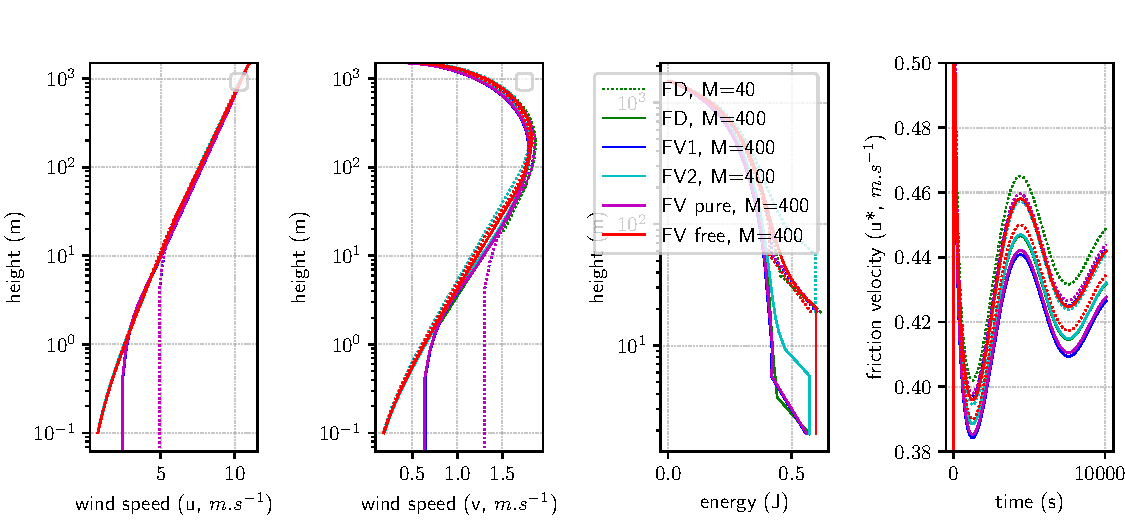
\includegraphics[scale=0.55]{images/consistency_comparison.pdf}
% 	\includegraphics[scale=0.55]{images/consistency_comparison_linearscale.pdf}
% 	\caption{Neutral case's numerical experiment. Top: log-scaled, bottom: linear-scaled}
% 	\label{fig:ND_NeutralCase_NumericalExp}
% \end{figure}
% \subsection{Variation of $\delta_{\rm sl}$}
% In this subsection we assume that $\delta_{\rm sl}$ can differ
% from one time to another. Let us note
% $\delta_{\rm sl}^n, \delta_{\rm sl}^{n+1}$ the two different sizes
% of the surface layer.
% There are 3 cases to take into account:
% \begin{enumerate}
% \item there is a $k$ such that
% 	$z_k< \delta_{\rm sl}^n, \delta_{\rm sl}^{n+1} < z_{k+1}$
% \item there is a $k$ such that
% 	$ \delta_{\rm sl}^n < z_k < \delta_{\rm sl}^{n+1}$
% \item there is a $k$ such that
% 	$ \delta_{\rm sl}^n > z_k > \delta_{\rm sl}^{n+1}$
% \end{enumerate}
% Note that multiple grid levels can be between $\delta_{\rm sl}^{n}$
% and $\delta_{\rm sl}^{n+1}$ in the second and third cases.
% \par
% Let $k^n$ be such that $z_{k^n} < \delta_{\rm sl}^{n}< z_{k^n + 1}$
% and $k^{n+1}$ such that
% $z_{k^{n+1}} < \delta_{\rm sl}^{n+1}< z_{k^{n+1} + 1}$
% \begin{enumerate}
% 	\item $k^n = k^{n+1}$:
% Since $\delta_{\rm sl}$ changes, then $\widetilde{h}$ also change.
% It must be taken into account when
% discretising in time the equations
% \eqref{eq:ND_NeutralCase_prognosticEqFVfree} and 
% \eqref{eq:ND_NeutralCase_semiDiscreteEkmanEqFVfree}.
% The boundary condition stays \eqref{eq:ND_NeutralCase_boundaryCondFVfree}.
% 	\item $k^n < k^{n+1}$:
% \eqref{eq:ND_NeutralCase_boundaryCondFVfree},
% \eqref{eq:ND_NeutralCase_prognosticEqFVfree} and 
% \eqref{eq:ND_NeutralCase_semiDiscreteEkmanEqFVfree} only need to
% be satisfied between $z_{k^{n+1}}$ and $z_{k^{n+1}+1}$.
% Hence, $\tau_{sl}(t^n)$ is set to 0.
% 	\item $k^n > k^{n+1}$:
% \eqref{eq:ND_NeutralCase_prognosticEqFVfree} and 
% \eqref{eq:ND_NeutralCase_semiDiscreteEkmanEqFVfree}
% need to be satisfied in both cells.
% {\color{red} It is not possible to do this in a natural way,
% because using \eqref{eq:ND_NeutralCase_prognosticEqFVfree}
% assumes the solution was a quadratic spline whereas it was actually
% a log profile.
% }
% \end{enumerate}
\paragraph{On the value of $K_{u,0}$}
\label{sec:ND_StratifiedCase_viscosity0_FVpure}
According to the wall law $K_{u,0}$ should be equal to $K_{mol}$.
However, the boundary condition $K_{u,0} \phi_0 = u_\star^2 e_\tau$
does not behave the same way with Finite Differences and Finite
Volumes.
\begin{itemize}
	\item \textbf{Finite Differences}:
Injecting the boundary condition at the first grid level gives
		\begin{equation}
			(\partial_t+if) u_{1/2} = \frac{1}{h_{1/2}}
			\left(K_{u,1}\frac{u_{3/2} - u_{1/2}}{h_1}
			 - \emphase{u_\star^2 e_\tau} \right)
		\end{equation}
The value of $K_0$ does not intervene in the equation.
\item \textbf{Finite Volumes} ("FV pure", "FV1" and "FV Nishizawa"):
Combining the equation \eqref{eq:ND_NeutralCase_prognosticEqFV}
and the reconstruction
\eqref{eq:ND_NeutralCase_quadraticReconstruction} in the second cell
$u(z_1) = {\cal S}_{\frac{3}{2}}\left(-\frac{h_\frac{3}{2}}{2}\right)$
the discretisations "FV pure", "FV1" and "FV Nishizawa"
implicitly use that
\begin{equation}
	(\partial_t+if) u(z_1) =
	\frac{K_{u,1} \phi_1 - \emphase{u_\star^2 e_\tau}}{h_{1/2}}
	+ (\partial_t+if)\left(\frac{\phi_1}{3}
	+ \emphase{\frac{u_\star^2 e_\tau}{6 K_{u,0}}}\right)h_{1/2}
\end{equation}
The (small) value of $K_{u,0}$ directly appears when we assume the
parabolic profile inside the first grid cell.
As a result, $u(z_1)$ scales with $\frac{1}{K_0}$ and
as it is seen in Figure \ref{fig:ND_NeutralCase_comparisonPlot}
exhibits unreasonable values.
To obtain physically plausible profiles,
by mimicking the relation
$\phi_{\delta} = \frac{K_{mol}}{K_{u,\delta}}\phi_0$ of the
"FV free" scheme, we choose to multiply the surface
viscosity by $\frac{K_{u,\delta}}{K_{mol}}$.
As a consequence, the wall law is denied and
$(\partial_z u)(z_0)$ is multiplied
by $\frac{K_{mol}}{K_{u,\delta}}$.
Note that this problem is specific to schemes where
$\frac{\phi_0}{K_{u,0}}$ is involved, and
is not characteristic of Finite Volume schemes.
\end{itemize}

\paragraph{In the general case where $\delta_{\rm sl} \geq z_k$.}
Let $k$ be such that $z_k \leq \delta_{\rm sl} < z_{k+1}$.
The surface layer scheme "FV free" is identical to the case $k=0$, except that
\begin{itemize}
	\item the sub-cell of average $\widetilde{u}$ and of size
		$\widetilde{h}$ is $[\delta_{\rm sl}, z_{\emphase{k+}1}]$:
		$k$ is added to the indices in 
		\eqref{eq:ND_NeutralCase_boundaryCondFVfree} and
		\eqref{eq:ND_NeutralCase_semiDiscreteEkmanEqFVfree};
	\item $\alpha_{sl} = \frac{\widetilde{h}}
			{h_{\emphase{k+}\frac{1}{2}}} +
		\frac{1}{h_{\emphase{k+}\frac{1}{2}}}
		\int_{z_\emphase{k}}^{\delta_{sl}}
		\frac{\ln(1+\frac{z}{z_{u}})}
			{\ln(1+\frac{\delta_{sl}}{z_{u}})} dz$;
	\item for $m < k$, the cell $[z_m, z_{m+1}]$ is filled with
		$K_{u,m} \phi_m = K_{u,k}\phi_k =
	{u_\star}^2e_\tau$
		and the average $\overline{u}_{m+1/2}$
		is computed with the integrated wall law
		between $z_m$ and $z_{m+1}$.
		The subgrid reconstruction in those cells is directly
		the wall law.
\end{itemize}
It is straightforward to check that for $\delta_{sl} = z_1$
the "FV2" scheme is rigorously recovered.
The derivation for any $\delta_{\rm sl} \geq 0$ is detailed for
the stratified case in Section \ref{sec:ND_StratifiedCase_FVfree}.
\begin{figure}
	\subimport{images/}{nouvelle_dis_neutre_anydelta.pdf_tex}
	\caption{ Surface layer scheme "FV free" with
	$\delta_{sl} \geq z_k$.}
	\label{fig:ND_NeutralCase_nouvelle_dis_neutre_anydelta}
\end{figure}
Figure \ref{fig:ND_NeutralCase_nouvelle_dis_neutre_anydelta}
shows how the surface layer is handled in this case: the part in gray
is neutralized for the prognostic equation and is filled afterward
with the help of the log law.
